Há 3 possibilidades para aproveitar a onda completa com um retificador a tiristor. Primeiro, como ilustra a figura \ref{pc}, um retificador em ponte utilizando somente tiristores.

\begin{figure}[h]
\center
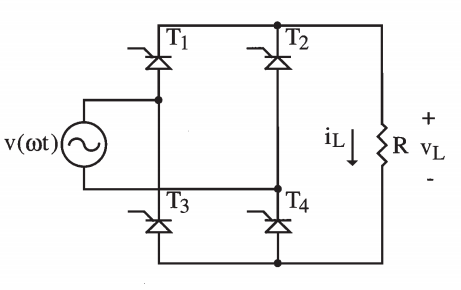
\includegraphics[scale=0.55]{imagens/ret_mono_comp_ponte.png}
\caption{Retificador de onda completa em ponte a tiristor.}\label{pc}
\caption*{Fonte: Eletrônica de potência (2006)}
\end{figure}

Essa é uma configuração relativamente redundante quanto ao controle, uma vez que não faz sentido o controle individual dos dois tiristores de cada par que compõe os possívei de entrar em condução a cada semiciclo. Dessa forma, surgem as configurações mistas da figura \ref{pma}, que associam tiristores e diodos em pares.

\begin{figure}[h]
\center
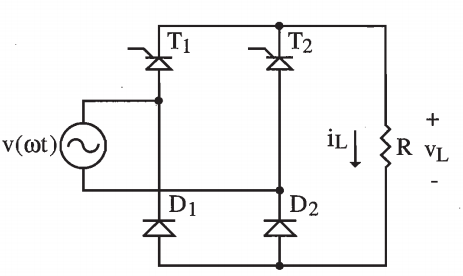
\includegraphics[width=0.45\textwidth]{imagens/ret_mono_comp_pontemista_a.png}
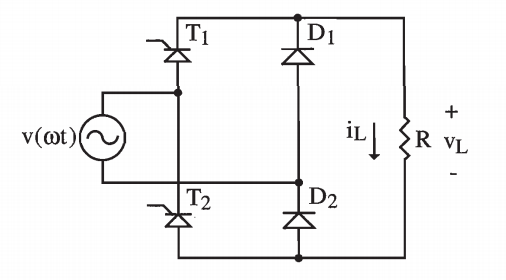
\includegraphics[width=0.45\textwidth]{imagens/ret_mono_comp_pontemista_b.png}
\caption{Retificador de onda completa com ponte mista A (esquerda) e B (direita).}\label{pma}
\caption*{Fonte: Eletrônica de potência (2006)}
\end{figure}

Por fim, há a configura com ponto médio tal qual a estudada para retificadores a diodo, como ilustra a figura \ref{pmed}. Novamente, destaca-se a necessidade de uma fonte simétrica como um secundário do transformador com uma conexão intermediária.

\begin{figure}[h]
\center
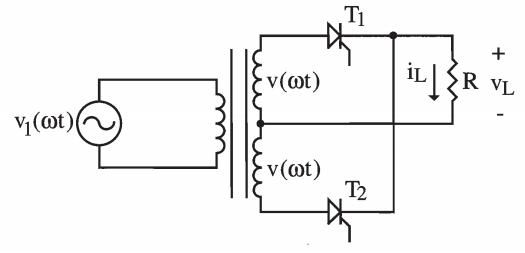
\includegraphics[scale=0.55]{imagens/ret_mono_comp_ponto_medio.png}
\caption{Retificador de onda completa a tiristor com ponto médio.}\label{pmed}
\caption*{Fonte: Eletrônica de potência (2006)}
\end{figure}

Ainda assim, o comportamento dessas implementações é o mesmo, como ilustra a figura \ref{gretr} no caso da carga resistiva, por isso serão estudados em conjunto.

\begin{figure}[h]
\center
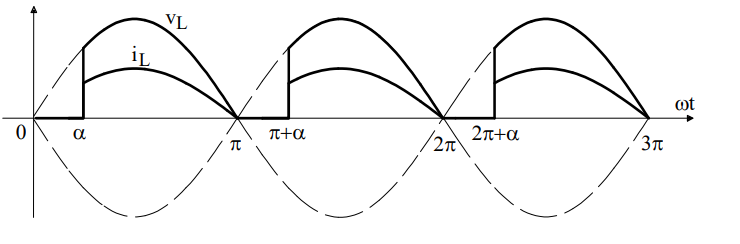
\includegraphics[scale=0.55]{imagens/grafico_ret_mono_comp.png}
\caption{Tensão e corrente em uma carga resistiva em um retificador de conda completa a tiristor.}\label{gretr}
\caption*{Fonte: Eletrônica de potência (2006)}
\end{figure}

Veja que até $\alpha$, quando um ou mais tiristores são ativados, a tensão na carga é nula. A partir desse momento, a tensão na carga (considerando o tiristor ideal) é tal qual a da alimentação. Assim, determinamos a tensão média
\begin{align*}
    V_{L,med} &= \frac{1}{\pi} \int_{0}^{\pi} \sqrt{2}V_{o}\sin(\omega{t})d(\omega{t})\\
&\approx 0,45V_{o}(1+\cos\alpha)
.\end{align*}
Verificamos que o resultado é condizente com a implementação a diodo uma vez que $\alpha=0$ implica na resposta já encontrada. Isso implica em uma relação entre a tensão média e o ângulo de disparo $\alpha$ como representada na figura \ref{gtmed}.

\begin{figure}[h]
\center
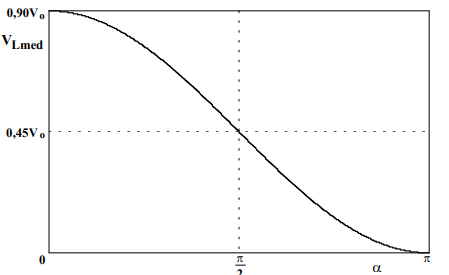
\includegraphics[scale=0.55]{imagens/ret_tensaomedia_resistivo.png}
\caption{Tensão média em função de $\alpha$ para carga resistiva no retificador de onda completa a tiristor.}\label{gtmed}
\caption*{Fonte:  EI I - Capitulo 3 - UNESP}
\end{figure}
\footnotetext{Disponível em: <www2.sorocaba.unesp.br/professor/flavioasg/ei/cap3.pdf> Acesso em set. 2018.}

Quando a carga possui componente indutivo é necessária a distinção entre as implementações. No caso do retificador totalmente controlado, tem-se o comportamento da tensão e da corrente na carga conforme ilustra a figura \ref{greti}. Aqui, utiliza-se:
\begin{description}
    \item[$\Delta$]  ângulo durante o qual a corrente de carga se mantém nula 
    \item[$\alpha$]  ângulo de disparo dos tiristores 
    \item[$\beta$] ângulo de extinção dos tiristores 
    \item[$\gamma$]  ângulo de condução
\end{description}

\begin{figure}[h]
\center
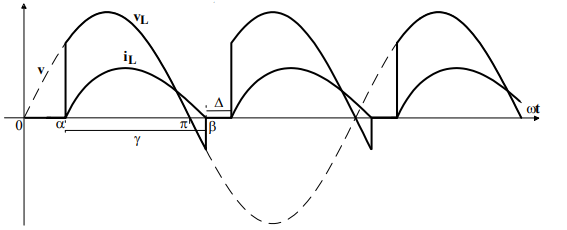
\includegraphics[scale=0.55]{imagens/grafico_ret_tensao_indutivo.png}
\caption{Tensão e corrente na carga com componente indutivo no retificador de onda completa a tiristor.}\label{greti}
\caption*{Fonte: Eletrônica de potência (2006)}
\end{figure}

Assim, a tensão média é
\begin{align*}
    V_{L,med} &= \frac{1}{\pi}\int_{0}^{\beta}\sqrt{2}V_{o}\sin(\omega{t})d(\omega{t}) \\
&\approx 0,45V_{o}(\cos\alpha - \cos\beta)
.\end{align*}

Já a corrente de carga pode ser determinada tal qual no retificador de meia onda a tiristor, ou seja, \[
i(\omega{t}) = \frac{\sqrt{2}V_{o}}{\sqrt{R^2+X^2}}[\sin(\omega{t}-\phi)-\sin(\alpha-\phi)e^\frac{-t'}{\tau}]
,\] onde $\phi = \arctan\frac{X}{R}$, $\tau = \frac{L}{R}$ e $t' =  t - \frac{\alpha}{\omega}$.

Veja que a condução é crítica se $\Delta = 0$ e, consequentemente, $\gamma = \pi$. A indutância crítica, que resulta na condução crítica, pode ser determinada sabendo-se que $i(\omega{t}) = 0$ quando $\beta = \pi + \alpha$, de forma que
\begin{align*}
 0 &= \sin(\pi+\alpha-\phi) - \sin(\alpha - \phi)e^{\frac{\pi}{\omega\tau}} \\
\omega\tau &= \frac{\omega{L}}{R} = \tan\phi \\
 \implies 0 &= \sin(\pi+\alpha-\phi) - \sin(\alpha - \phi)e^{\frac{\pi}{\tan\phi}}
.\end{align*}

Uma vez que essa igualdade só é válida para $\alpha=\phi$, pode-se substituir esse valor em $\omega\tau = \frac{\omega{L}}{R} = \tan\phi$ para determinar o valor da indutância crítica.

No caso de condução descontínua, $\omega{t}=\beta \implies i(\omega{t})=0$. Assim,
\begin{align*}
 0 &= \sin(\beta-\phi) - \sin(\alpha - \phi)e^{\frac{t'}{\tau}} \\
t' &= t - \frac{\alpha}{\omega} = \frac{\omega{t}}{\omega} - \frac{\alpha}{\omega} = \frac{\beta-\alpha}{\omega} \\
 \implies 0 &= \sin(\beta-\phi) - \sin(\alpha - \phi)e^{\frac{\beta-\alpha}{\tan\phi}}
.\end{align*}
De forma numérica, é possível determinar $\beta$ a partir de $\alpha$ e $\phi$.

Agora, podemos ver que o ângulo da tensão média, fixando-se $\alpha, \omega, V_{o}$ e L, depende apenas da resistência R da carga. Essa relação é ilustrada pela figura \ref{gretioc0}.

\begin{figure}[h]
\center
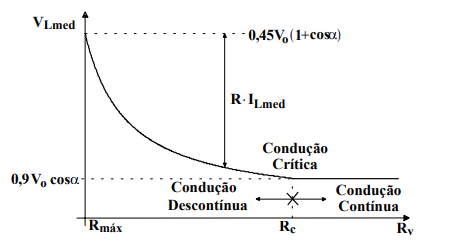
\includegraphics[scale=0.75]{imagens/grafico_ret_carga_indutivo.png}
\caption{Relação entre a tensão média e o componente resistivo da carga em um retificador de onda completa em ponte a tiristor.}\label{gretioc0}
\caption*{Fonte: EI I - Capitulo 3 - UNESP}
\end{figure}

Em condução descontínua, podemos modelar o retificador como uma fonte ideal em série com uma resistência variável pela corrente $I_{L,med}$, como ilustrado na figura \ref{cgretioc}.

\begin{figure}[h]
\center
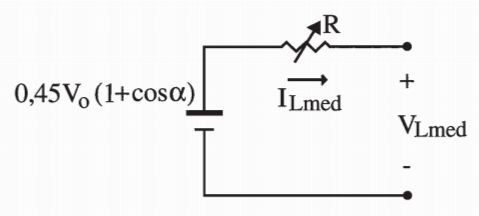
\includegraphics[scale=0.55]{imagens/circuito_equevalente.png}
\caption{Circuito equivalente de saída para o retificador de onda completa a tiristor.}\label{cgretioc}
\caption*{Fonte: Eletrônica de potência (2006)}
\end{figure}

Já no caso da condução contínua,
\begin{align*}
\beta &= \pi + \alpha \\
\implies V_{L,med} &= 0,45V_{o}(\cos\alpha - \cos\beta) \\
&= 0,45V_{o}[\cos\alpha - \cos(\pi+\alpha)] \\
&= 0,9V_{o}\cos\alpha
,\end{align*}
comportamento ilustrado na figura \ref{gretinv}.

\begin{figure}[h]
\center
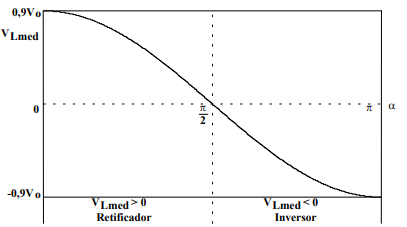
\includegraphics[scale=0.55]{imagens/grafico_ret_inversor.png}
\caption{Gráfico da tensão média para o retificador de onda completa com carga indutiva em condução contínua.}\label{gretinv}
\caption*{Fonte:  EI I - Capitulo 3 - UNESP}
\end{figure}

Uma vez que a corrente é sempre positiva, podemos determinar o fluxo de potência entre a fonte e a carga através da tensão média, ou seja, quando essa é negativa, o circuito se torna um retificador. Esse fenômeno, característico do circuito da figura \ref{cretoc}, está ilustrado na figura \ref{gretiocb}. Ressalta-se que esse inversor só funciona para corrente alternada.

\begin{figure}[h]
\center
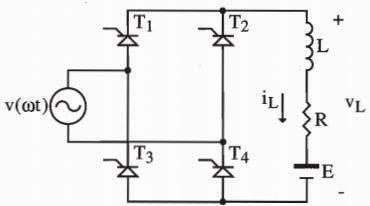
\includegraphics[scale=0.55]{imagens/circuito_ret_inversor.png}
\caption{Retificador de onda completa a tiristor atuando como inversor.}\label{cretoc}
\caption*{Fonte: Eletrônica de potência (2006)}
\end{figure}

\begin{figure}[h]
\center
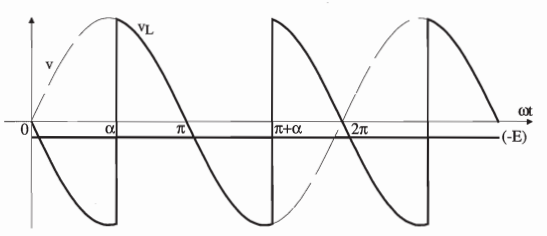
\includegraphics[scale=0.55]{imagens/grafico_conversor_inv.png}
\caption{Tensão da carga indutiva em um retificador de onda completa a tiristor atuando como inversor.}\label{gretiocb}
\caption*{Fonte: Eletrônica de potência (2006)}
\end{figure}

Tais retificadores totalmente controlados, que podem operar como inversores não autônomos, são bastante utilizados, por exemplo, em transmissão de energia elétrica a corrente contínua, tanto a retificação quanto a inversão, uma vez que podem ser feitas ambas por esse componente.

Já no caso do retificador com ponte mista, os diodos atuam, naturalmente como diodos de roda livre, como ilustra a figura \ref{epm}.

\begin{figure}[h]
\center
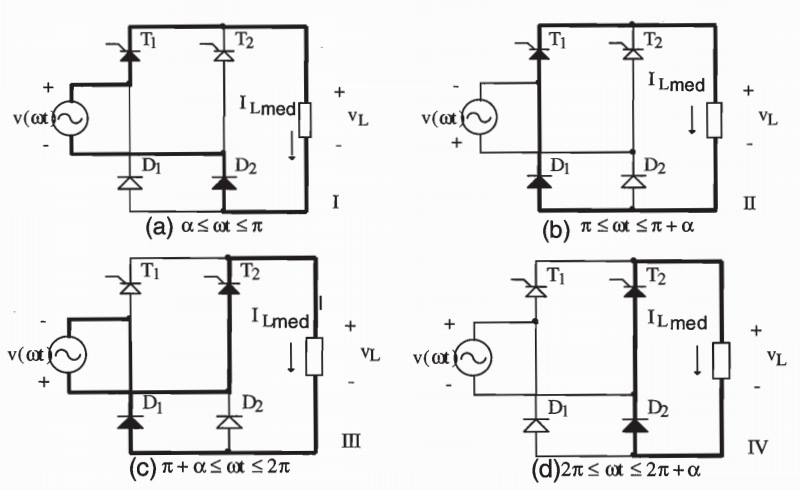
\includegraphics[scale=0.55]{imagens/etapas_ponte_mista.png}
\caption{Comportamento do retificador de onda completa com ponte mista com uma carga com componente indutivo.}\label{epm}
\caption*{Fonte: Eletrônica de potência (2006)}
\end{figure}

Da mesma forma, a tensão média é 
\begin{align*}
 V_{L,med} &= \frac{1}{\pi}\int_{\alpha}^{\pi}\sqrt{2}V_{o}\sin(\omega{t}d(\omega{t}) \\
 &= 0,45V_{o}[1+\cos(\alpha)]
.\end{align*}
Fica claro que essa configuração não funciona como um inversor.

